\chapter{Povezani i sli�ni radovi}

Osim paleta komandi prisutnih u ure�iva�ima koda kao �to su \textit{Atom}, \textit{Sublime Text} o \textit{Visual Studio Code}, postoje i ostali sli�ni primjeri koji za cilj imaju olak�anu pretragu za naredbama neke aplikacije ili ubrzavanje rada za ra�unalom na neki drugi na�in.

\section{Unity HUD, Plotinus i Gnome HUD}

\begin{figure}[!htbp]
	\begin{center}
		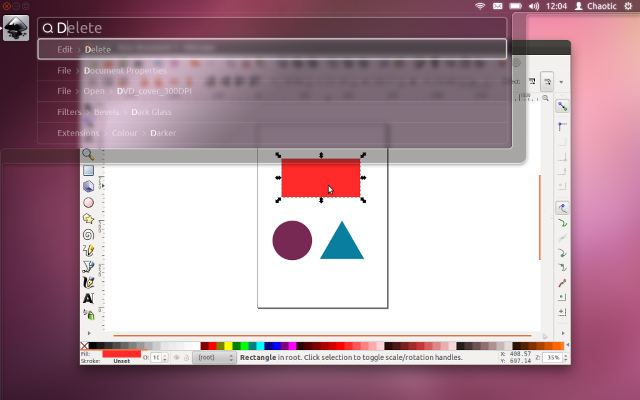
\includegraphics[scale=0.7]{unity_hud}
		\caption{Unity HUD}
		\label{fig:unity_hud}
	\end{center}
\end{figure}

Kao proizvod koji je najsli�niji univerzalnoj paleti komandi name�e se \textbf{Unity HUD} \cite{11_2019}, prisutan u grafi�koj ljusci za Linux operacijske sustave \textbf{Unity}. Unity HUD mo�e raditi na vi�e razli�itih programa, odnosno nije eksplicitno implementiran za to�no odre�ene aplikacije. Automatski u�itava naredbe iz izbornika trenutno fokusiranog programa te nudi mogu�nost njihovog pretra�ivanja i uporabe, �to se mo�e vidjeti na slici \ref{fig:unity_hud} \cite{11_2019}. Unity HUD tako iskori�tava su�elje koje nude aplikacije na Ubuntu sustavima iz kojih mo�e saznati stavke koje se nalaze u njihovim izbornicima.

Me�utim, ovaj program ima sljede�e nedostatke:

\begin{itemize}
\item Zbog na�ina implementacije ne mo�e se koristiti na Windows operacijskim sustavima (usko je vezan uz arhitekturu Linux aplikacija)
\item Unity ljuska za GNOME nije vi�e u aktivnom razvoju od strane njenog autora, tvrtke Canonical \cite{12_2019}
\end{itemize}

\begin{figure}[!htbp]
	\begin{center}
		\includegraphics[scale=0.7]{Plotinus}
		\caption{Plotinus}
		\label{fig:plotinus}
	\end{center}
\end{figure}

Sli�no rje�enje je i \textbf{Plotinus}, vidljiv na slici \ref{fig:plotinus} \cite{13_2019} koji, uz �injenicu da nije u aktivnom razvoju (zadnje osvje�enje se dogodilo 4.6.2017. godine) tra�i i ru�nu konfiguraciju odre�enih sistemskih datoteka, �to predstavlja prepreku za korisnike koji nemaju tehni�ka znanja za rad u Linux sustavima. Tako�er, kao i u slu�aju Unity HUD-a, Plotinus mo�e biti kori�ten samo na Linuxu.

\begin{figure}[!htbp]
	\begin{center}
		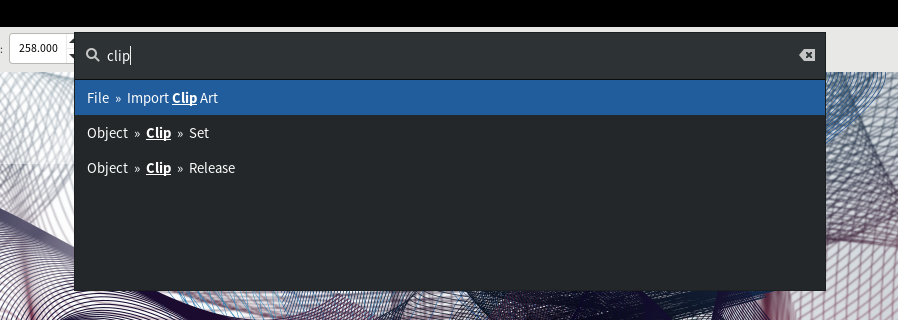
\includegraphics[scale=1.95]{gnome_hud}
		\caption{Gnome HUD}
		\label{fig:gnome_hud}
	\end{center}
\end{figure}

Naposljetku, Gnome HUD, prikazan na slici \ref{gnome_hud} \cite{14_2019} se redovitije osvje�ava i tra�i manje konfiguracije, no svejedno je potrebno instalirati dodatne pakete za potpunu kompatibilnost s GTK i Qt alatima za izradu grafi�kih su�elja.

\section{Microsoft Word pretra�ivanje naredbi}